\begin{frame}{Qualitative results: Our system}
  % Show some impressive qualitative results that are better than naive
  % initialization
  \centering
  \includemedia[label=allenergies,
    width=\linewidth,height=0.6\linewidth, % 16:9
    activate=pageopen,
    addresource=graphics/allenergies_2.mp4,
    flashvars={
      source=graphics/allenergies_2.mp4
      &loop=true             % loop video
      &scaleMode=letterbox   % preserve aspect ratio while scaling the video
    }
  ]{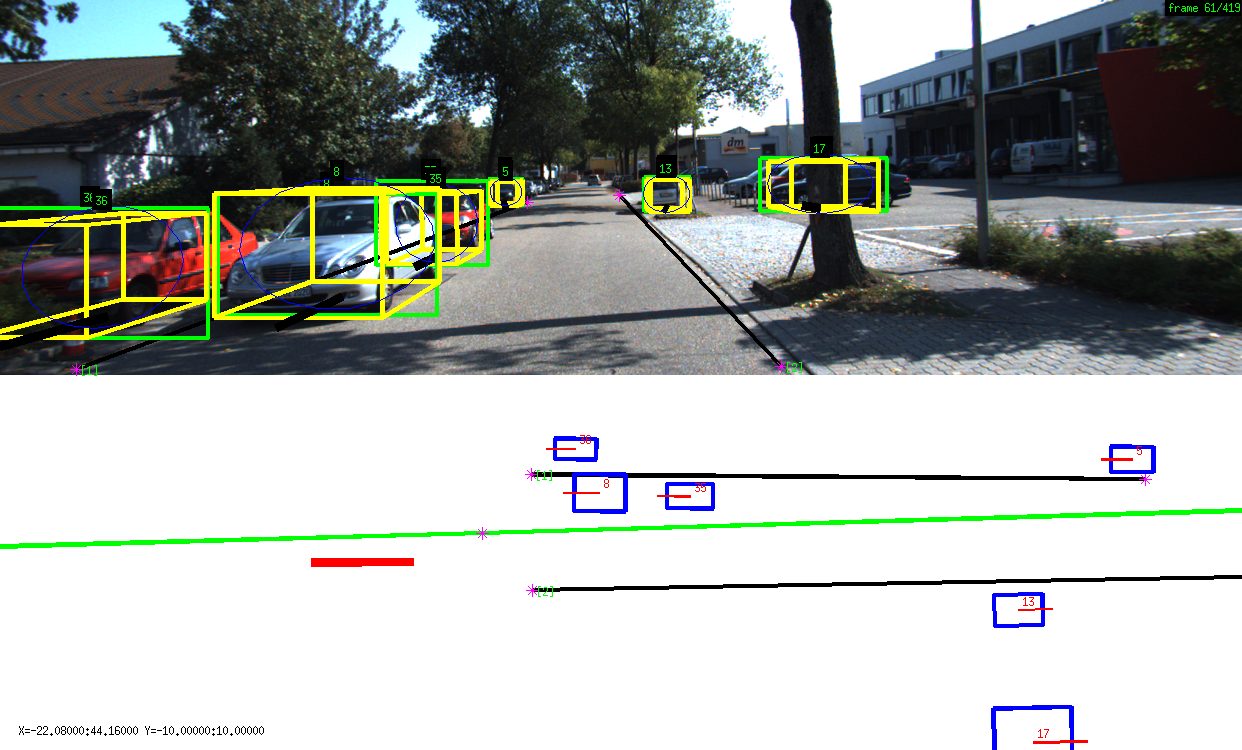
\includegraphics{graphics/0000000061_bevdown.png}}{VPlayer.swf}
\end{frame}

\begin{frame}{Quantitative results}

  \begin{tabular}{lrr}
    \toprule
    Method & t & dim \\
    \midrule
    Point cloud fit
    & 6.87 & 4.02\\
    Initialization
    & 5.61 & 3.23\\
    $\EnergyTrackNoOcc + \EnergyBBoxNoOcc +\EnergySize+\EnergyDyn$ 
    & 3.95  & 1.72\\        
    $\EnergyTrackNoOcc + \EnergyBBox +\EnergySize+\EnergyDyn$        
    & 4.81  & 2.16\\        
    $\EnergyTrack + \EnergyBBoxNoOcc +\EnergySize+\EnergyDyn$      
    & 4.05  & {\bf 1.59}\\        
    $\EnergyTrack + \EnergyBBox +\EnergySize+\EnergyDyn$             
    & {\bf 3.24}  & 2.16\\
    \bottomrule
  \end{tabular}
  
\end{frame}

\begin{frame}{Future work}
  \begin{itemize}
    \item Speedup inference
    \item Simplify graph by \cite{chow1968approximating} tree approximation
    \item Use belief propagation for faster inference on trees
  \end{itemize}
  
\end{frame}

\begin{frame}{Conclusion}
    Our occlusion aware 3D modeling improves association\\
    ... but requires more work to show improvement on localization
\end{frame}
